
\documentclass [PhD] {uclathes}

% \input {mymacros}                         % personal LaTeX macros
\usepackage[round]{natbib}
\def\newblock{\ }
\usepackage[T1]{fontenc}
\usepackage{times}
\usepackage{latexsym}
\usepackage[utf8]{inputenc}
\usepackage{graphicx}
\usepackage{multirow}
\usepackage{microtype}
\usepackage{inconsolata}
\usepackage{subcaption}
\usepackage{amsfonts,amssymb}
\usepackage{booktabs}


%%%%%%%%%%%%%%%%%%%%%%%%%%%%%%%%%%%%%%%%%%%%%%%%%%%%%%%%%%%%%%%%%%%%%%
%
% Usually things live in separate flies.
%
% \input {prelim}                           % preliminary page info

%%%%%%%%%%%%%%%%%%%%%%%%%%%%%%%%%%%%%%%%%%%%%%%%%%%%%%%%%%%%%%%%%%%%%%%%
%                                                                      %
%                          PRELIMINARY PAGES                           %
%                                                                      %
%%%%%%%%%%%%%%%%%%%%%%%%%%%%%%%%%%%%%%%%%%%%%%%%%%%%%%%%%%%%%%%%%%%%%%%%

\title          {Mitigating Gender and Racial Bias \\
                in Automated English Speaking Assessmenth}
\author         {Alexander Kwako}
\department     {Education}
% Note:  degreeyear should be optional, but as of  5-Feb-96
% it seems required or you get a year of ``2''.   -johnh
\degreeyear     {2023}

%%%%%%%%%%%%%%%%%%%%%%%%%%%%%%%%%%%%%%%%%%%%%%%%%%%%%%%%%%%%%%%%%%%%%%%%

\chair          {Michael\ Seltzer}
\member         {Mark Hansen}
\member         {Li\ Cai}
\member         {Kai-Wei\ Chang}

%%%%%%%%%%%%%%%%%%%%%%%%%%%%%%%%%%%%%%%%%%%%%%%%%%%%%%%%%%%%%%%%%%%%%%%%

\dedication     {\textsl{To my mother \ldots \\
                who---among so many other things--- \\
                saw to it that I learned to touch-type \\
                while I was still in elementary school}}

%%%%%%%%%%%%%%%%%%%%%%%%%%%%%%%%%%%%%%%%%%%%%%%%%%%%%%%%%%%%%%%%%%%%%%%%

\acknowledgments {(Acknowledgments omitted for brevity.)}

%%%%%%%%%%%%%%%%%%%%%%%%%%%%%%%%%%%%%%%%%%%%%%%%%%%%%%%%%%%%%%%%%%%%%%%%

\vitaitem   {1974--1975}
                {Campus computer center ``User Services'' programmer and
                consultant, Stanford Center for Information Processing,
                Stanford University, Stanford, California.}
\vitaitem   {1974--1975}
                {Programmer, Housing Office, Stanford University.
                Designed a major software system for assigning
                students to on-campus housing.
                With some later improvements, it is still in use.}
\vitaitem   {1975}
                {B.S.~(Mathematics) and A.B.~(Music),
                Stanford University.}
\vitaitem   {1977}
                {M.A.~(Music), UCLA, Los Angeles, California.}
\vitaitem   {1977--1979}
                {Teaching Assistant, Computer Science Department, UCLA.
                Taught sections of Engineering 10 (beginning computer
                programming course) under direction of Professor Leon
                Levine.
                During summer 1979, taught a beginning programming
                course as part of the Freshman Summer Program.}
\vitaitem   {1979}
                {M.S.~(Computer Science), UCLA.}
\vitaitem   {1979--1980}
                {Teaching Assistant, Computer Science Department, UCLA.}
\vitaitem   {1980--1981}
                {Research Assistant, Computer Science Department, UCLA.}
\vitaitem   {1981--present}
                {Programmer/Analyst, Computer Science Department, UCLA.}

%%%%%%%%%%%%%%%%%%%%%%%%%%%%%%%%%%%%%%%%%%%%%%%%%%%%%%%%%%%%%%%%%%%%%%%%

\publication    {\textsl{MADHOUS Reference Manual.}
                Stanford University, Dean of Student Affairs
                (Residential Education Division), 1978.
                Technical documentation for the MADHOUS
                software system used to assign students to
                on-campus housing.}

%%%%%%%%%%%%%%%%%%%%%%%%%%%%%%%%%%%%%%%%%%%%%%%%%%%%%%%%%%%%%%%%%%%%%%%%

\abstract{
In English speech assessment, pretrained large language models (LLMs) such as BERT have been shown to score responses as accurately as human raters. Yet it remains unknown whether BERT perpetuates or exacerbate biases, which could pose problems for the fairness and validity of the test. This study examines gender and native language (L1) biases in human and BERT-based automated scores in a large-scale, K-12 English speaking assessment. Analyses of bias focus on differential item functioning (DIF). Results show that, with respect to examinees’ L1 background, there is a moderate amount of DIF, and this DIF is higher when scored by an off-the-shelf BERT model. In practical terms, the degree to which BERT exacerbates DIF is very small. There is more DIF for longer speaking items and for older examinees, but BERT does not exacerbate these patterns of bias. 
}

%%%%%%%%%%%%%%%%%%%%%%%%%%%%%%%%%%%%%%%%%%%%%%%%%%%%%%%%%%%%%%%%%%%%%%%%



\begin {document}
\makeintropages

%%%%%%%%%%%%%%%%%%%%%%%%%%%%%%%%%%%%%%%%%%%%%%%%%%%%%%%%%%%%%%%%%%%%%%
%
% Ordinarily each chapter (at least) is in a separate file.
%
%\input {chapter1}                         % Chapter 1 of dissertation
%\input {chapter2}                         % Chapter 2
%\input {chapter3}                         % etc.
%\input {chapter4}
%\input {chapter5}
%\input {chapter6}
%\input {chapter7}
%\input {chapter8}

\chapter{Introduction}

Pretrained large language models (LLMs) present new opportunities for English speaking assessments, yet they are prone to perpetuating (and in some cases exacerbating) social prejudices \citep{blodgett2020}. In educational assessment, researchers have shown that pretrained LLMs can replicate human scoring, including English speech assessment, with a high degree of accuracy \citep{wang2021automated}. Studying biases of these automated scoring systems, however, is uncommon \citep{ormerod2022short}. Considering how widespread and high stakes English speaking assessments are at both the primary and secondary education levels \cite{cimpian2017, ets2005}, it is imperative that these assessments be fair for all students, regardless of gender or L1 backgrounds. This study addresses the need for deeper analyses of bias in LLM-based automated English speaking assessments. 

\section{Bias in English speaking assessment}

\noindent \textbf{Human rater bias}\; 
Scholarship on implicit bias demonstrates that human judgment is influenced unconsciously by peripheral cues, including speakers’ accents \citep{kang2021social}. In the context of English speaking assessment, these biases may lead to unfair scoring without raters even realizing it \citep{greenwald1995}. Indeed, \citet{winke2013} reports that human raters are more lenient towards examinees who share the same L1 background. In a summary of research on the biases of raters of L2 English, \citet{lindemann2013reliably} reports a strong disconnect between subjective evaluation of speech (e.g. using Likert scales) and more objective measures (e.g. transcription). 

Research on implicit bias and speech suggests that, in the context of English language assessment, there may be more bias in the domain of Speaking (e.g. as opposed to Writing). By listening to examinees’ voices, human raters may be more likely to be influenced by examinees’ accents, triggering implicit bias that affects their judgment during scoring.

\noindent \textbf{Transcription bias}\; 
Another potential source of bias in automated speaking assessment is automated transcription. Anonymous has shown that the largest providers of automated transcription services (Google, Amazon, and Microsoft) all have discrepancies in transcription accuracy based on speakers’ L1. As text transcripts constitute the most important (if not exclusive) input for most pretrained LLM scoring systems, it is important to consider that systematic discrepancies in transcripts may lead to systematic discrepancies in scores.

\noindent \textbf{Socio-cultural factors}\; 
There are many socio-cultural differences based on gender and L1 that affect English speaking assessment. \citet{derwing2013development}, for instance, discuss how factors like age and conversational opportunities interact with L1 in complex ways. Gender is also a source of variation in L2 English speaking proficiency, although it varies by culture and task \citep{denies2022mapping}. 

\subsection{LLMs may exacerbate social biases}

Studies have revealed that pretrained LLMs can propagate and, in some cases, amplify negative stereotypes of marginalized groups \citep{blodgett2020}. Because LLMs are pretrained on large corpora of text, largely scraped from the web, societal biases in these texts become embedded in the LLMs. These biases may surface in downstream applications, such as machine translation \citep{stanovsky2019evaluating} and sentiment analysis \citep{kiritchenko2018examining}. 

In English speaking assessment, LLMs are not yet in widespread use. Yet researchers who are exploring their use typically focus on performance metrics (e.g. accuracy) to the exclusion of analyses of bias \citep[e.g.][]{wang2021automated}. In NLP-based English speaking assessment more broadly, Even among NLP-based speaking assessments that are in production, analyses of bias are rarely conducted or reported \citep[e.g. ][]{collier2020test}. In one rare study, however, \citet{wang2018monitoring} found that their automated scoring system diverged from human raters for several L1 groups.  

\subsection{Differential item functioning (DIF)}
\label{intro_dif}

Differential item functioning (DIF) is a specific type of bias commonly examined in educational and psychological assessment \citep{aera2014}. DIF occurs when “equally able (or proficient) individuals, from different groups, do not have equal probabilities of answering the item correctly” \citep[][p. 4]{angoff1993}. 

Although there are many studies of DIF with respect to gender and L1 in large-scale English language assessment, these studies focus on vocabulary, listening, and writing proficiency \citep{kunnan2017evaluating}. Very few studies of DIF have been conducted on English speaking proficiency. 

\subsection{Study overview and research questions}

This study is designed to analyze gender and L1 biases in a pretrained LLM-based automated English speaking assessment. Our data come from a large-scale K-12 English language assessment known as the English Language Proficiency Assessment for the 21st Century \citep[ELPA21;][]{huang2018english}. We focus on speaking proficiency in particular, since it is more susceptible to implicit bias than other domains of English language proficiency. For our automated scoring model, we use an off-the-shelf pretrained Bidirectional Encoding Representation using Transformers \citep[BERT;][]{devlin2018} because it is a seminal architecture and remains a focus of study in English speaking assessment \citep{wang2021automated}. We quantify the amount of bias in human and automated scores by calculating DIF. We describe specific patterns of DIF in human scores, and determine whether or not BERT exacerbates DIF. Specifically, our study addresses the following specific research questions:

\begin{enumerate}
    \item Compared to human scores, does BERT increase overall DIF with respect to gender or L1?
    \item Does DIF increase with item length and, if so, is this exacerbated by BERT?
    \item Is DIF higher for older examinees and, if so, is this exacerbated by BERT?
    \item Which specific groups of examinees are (dis)advantaged most, and does BERT exacerbate these (dis)advantages?
\end{enumerate}

\chapter{Methods}

\subsection{Data}

This study draws on data from the English Language Proficiency Assessment for the 21st Century (ELPA21), a consortium involving 7 state education agencies in the U.S. \citep{huang2018english}. To maintain confidentiality, certain details regarding test items and examinees are omitted. 

Analyses focused on two grade-bands (2–3 and 9–12) which corresponded to two tests administered during the 2020–2021 school year. For items in the Speaking domain, examinees spoke into a microphone for up to two minutes, after which their responses were sent to human raters who assigned holistic integer scores based on item-specific scoring rubrics. All verbal responses in ELPA21 are currently scored by human raters Raters are trained and monitored over time to ensure consistency \citep{engelhard2002monitoring}. 

\subsection{Sample design and demographics}

The sampling frame included all examinees in grade-bands in 2–3 or 9–12 who met the following inclusion criteria: answered all three speaking items included in this study; answered enough items in each of the other three domains to receive domain-specific scores; and had gender and L1 demographic information available. Furthermore, to limit the scope of the study, we excluded examinees who had an IEP or 504 Plan, examinees with non-binary gender, and examinees whose L1 was other than one of the ten L1s analyzed in this study. 

From the sampling frame, we sampled 15,000 students.\footnote{The size of our sample was limited, in part, by the cost of automated transcription.} We included all examinees whose L1 was one of the nine L1 focal groups (Table \ref{smp_dscr}). The remainder of examinees were randomly sampled from Spanish speakers. 

\begin{table*}[htbp]
\centering
% \small  % comment out this line if wanted bigger font size
\begin{tabular}{lccccccc}
\toprule
    & \multicolumn{3}{c}{\textbf{Grade Band 2-3}} & \multicolumn{1}{c}{ } & \multicolumn{3}{c}{\textbf{Grade Band 9-12}} \\
    \cline{2-4}
    \cline{6-8}
     & \textbf{n} & \textbf{\%} & \textbf{Avg. Proficiency} & & \textbf{n} & \textbf{\%} & \textbf{Avg. Proficiency} \\
    \midrule
    \textbf{All} & 8377 & 100 & 0.18 (0.91) & & 6623 & 100 & 0.16 (0.93) \\
    \textbf{Gender} &  &  &  & &  &  &  \\
    \hspace{3mm} Male & 4310 & 51.5 & 0.13 (0.9) & & 3648 & 55.1 & 0.14 (0.94) \\
    \hspace{3mm} Female & 4067 & 48.5 & 0.23 (0.92) & & 2975 & 44.9 & 0.2 (0.92) \\
    \textbf{L1} &  &  &  & &  &  &  \\
    \hspace{3mm} Spanish & 4205 & 50.2 & 0.08 (0.85) & & 3481 & 52.6 & 0.23 (0.92) \\
    \hspace{3mm} Marshallese & 692 & 8.3 & -0.0 (0.86) & & 891 & 13.5 & -0.05 (0.75) \\
    \hspace{3mm} Russian & 862 & 10.3 & 0.28 (0.9) & & 375 & 5.7 & 0.49 (0.86) \\
    \hspace{3mm} Vietnamese & 522 & 6.2 & 0.41 (0.9) & & 402 & 6.1 & 0.36 (0.93) \\
    \hspace{3mm} Arabic & 499 & 6 & 0.33 (0.88) & & 414 & 6.3 & 0.06 (0.86) \\
    \hspace{3mm} Mandarin & 439 & 5.2 & 0.88 (0.89) & & 203 & 3.1 & 0.44 (1.02) \\
    \hspace{3mm} Hindi & 416 & 5 & 0.75 (0.82) & & 185 & 2.8 & 0.67 (0.82) \\
    \hspace{3mm} Mayan & 238 & 2.8 & -0.66 (0.88) & & 258 & 3.9 & -0.84 (0.95) \\
    \hspace{3mm} Persian & 295 & 3.5 & -0.05 (1.01) & & 197 & 3 & -0.07 (0.94) \\
    \hspace{3mm} Swahili & 209 & 2.5 & 0.22 (0.87) & & 217 & 3.3 & 0.04 (0.93) \\
    \bottomrule
    \end{tabular}
\caption{\label{smp_dscr}
Sample descriptive statistics in aggregate ("All") and disaggregated by gender and L1.}
\end{table*}

Demographics of grade-bands 2–3 and 9–12 are presented in Table \ref{smp_dscr}. Note that there are group differences with respect to overall language proficiency.\footnote{See Section \ref{meth_dif} for how language proficiency is computed for examinees.} In both grade-bands, male examinees scored slightly lower than female examinees. There is also heterogeneity among L1 groups.

\subsection{L1 selection}

Due to practical limitations, we focused on ten L1 groups. Spanish was the largest L1 group (constituting 82.7\% of all examinees in 2020–2021) and, for this reason, served as the reference group. The other nine L1 groups were selected based on the number of examinees available, and with a view to global diversity. See Appendix \ref{sec:appendix_lang} for additional details regarding L1 selection and grouping.

\subsection{Item selection}

Speaking items were selected to span a range of response times (i.e., length or quantity of speech). Specifically, for each grade-band, we selected one speaking item that was short in duration (i.e., requiring examinees to produce a phrase or simple sentence to answer the prompt), one medium-length item (i.e., requiring 2–3 sentences or a compound sentence), and one long item (i.e., requiring 3+ sentences). Table \ref{itm_dscr} presents the lengths of items 1–3, based on average audio duration (in seconds) and average number of words, for both grade-bands. To increase comparability between grade-bands, our selection of items also took into consideration item type and item information. 

\begin{table*}[ht]
\centering
% \small  % comment out this line if wanted bigger font size
\begin{tabular}{llccccccc}
\toprule
    & & \multicolumn{3}{c}{\textbf{Grade Band 2-3}} & \multicolumn{1}{c}{ } & \multicolumn{3}{c}{\textbf{Grade Band 9-12}} \\
    \cline{3-5}
    \cline{7-9}
     % \textbf{Item #} & \textbf{Length} & \textbf{Num. Categories} & \textbf{Avg. Seconds} & \textbf{Avg. Words} & & \textbf{Num. Categories} & \textbf{Avg. Seconds} \\
     \textbf{Item \#} & \textbf{Length} & \multicolumn{1}{p{1.5cm}}{\centering \textbf{Num. of} \\ \textbf{categories}} & \multicolumn{1}{p{1.5cm}}{\centering \textbf{Avg.} \\ \textbf{seconds}} & \multicolumn{1}{p{1.5cm}}{\centering \textbf{Avg.} \\ \textbf{words}} & & \multicolumn{1}{p{1.5cm}}{\centering \textbf{Num. of} \\ \textbf{categories}} & \multicolumn{1}{p{1.5cm}}{\centering \textbf{Avg.} \\ \textbf{seconds}} & \multicolumn{1}{p{1.5cm}}{\centering \textbf{Avg.} \\ \textbf{words}} \\
    \midrule
    Item 1 & short & 3 & 6.4 (4.9) & 6.0 (6.5) & & 4 & 8.3 (5.0) & 11.5 (7.1) \\
    Item 2 & medium & 5 & 17.2 (13.3) & 25.1 (23.2) & & 6 & 14.9 (9.1) & 22.8 (16.7) \\
    Item 3 & long & 6 & 36.9 (23.1) & 51.1 (35.0) & & 5* & 34.7 (18.9) & 65.0 (38.4) \\
    \bottomrule
    \end{tabular}
\caption{\label{itm_dscr}
Item descriptive statistics. Item 3 for grade-band 9–12 was re-scaled from a 6-point scale to a 5-point scale. This change was made due to the fact that one group of respondents (Hindi) did not receive any 1s. Combining 1s with 2s helped to improve model convergence.}
\end{table*}

\subsection{Automated Transcription}

Automated transcripts were generated using Amazon Web Services, during October 7–12 and November 14–16, 2022. Default transcription settings were used, with output language set to “en-US.” Amazon provides multiple transcripts by default; the most probable transcripts were selected for analyses.

The accuracy and biases of Amazon’s automated transcription service are reported in Anonymous. Briefly, results showed that overall word error rate (WER) was 18.5\%, on par with human-human levels of agreement for L2 English speech \citep{zechner2009}. The WER of examinees in grade-band 2–3 was, on average, higher than the WER of examinees in grade-band 9–12 (20.5\% versus 16.5\%, respectively). We found no evidence of gender biases when controlling for overall language proficiency; yet we found that Vietnamese speakers had a higher WER than other L1 groups (24.0\%, on average), and Arabic speakers had a lower WER (12.6\%). 

\subsection{Differential item functioning (DIF)}
\label{meth_dif}

As discussed in Section \ref{intro_dif}, DIF occurs when there are group differences, conditional on unbiased proficiency estimates. The unbiased proficiency estimate, $\theta$, is referred to as the \emph{matching criterion}. In this study, the matching criterion is examinees’ non-Speaking English language proficiency, inferred from a unidimensional IRT model. By excluding speaking items, we ensured that estimates of $\theta$ were not contaminated by the same type(s) of bias under examination. 

The majority group is referred to as the \emph{reference group}; and the minority group is referred to as the \emph{focal group}. For gender, the reference group was Male (and the focal group was Female); for L1, the reference group is Spanish (and the nine focal groups are listed in Table \ref{smp_dscr}). 

\subsection{DIF effect sizes}
\label{meth_fx}

As summarized by \cite{michaelides2008}, a common method to evaluate DIF for ordinal items is based on the standardized mean difference (SMD) between reference and focal groups \citep{dorans1986}.\footnote{Instead of using the Mantel test \citep{mantel1963}, our significance tests are based on bootstrap sampling distributions and B-H adjusted $p$-values, described in Sections \ref{meth_boot} and \ref{meth_bh}.} The effect size, $z$, is the ratio of SMD to the standard deviation (pooled between the two groups).\footnote{\cite{ormerod2022automated} refer to the effect size as $z$, a convention we follow.} Intuitively, $z$ represents how much the focal group outperforms the reference group, comparing examinees of similar proficiency,\footnote{Examinees were divided into ten strata based on which quantile of the standard normal distribution their non-Speaking English proficiency resided.} in units of standard deviation. 

What counts as a large or small effect size is based on a system originally proposed by \citet{zwick1993assessment} and is used by the Educational Testing Service and other educational assessment organizations. Generalizing the system to ordinal items, \citet[][p. 150]{naep2001} designates items as having strong DIF (labeled “CC”) if z is greater than or equal to 0.25. Items have weak DIF (“AA”) if z is less than 0.17. And items have moderate DIF (“BB”) if z is between 0.17 and 0.25. 

\noindent \textbf{Absolute effect size} \;
For certain research questions, the primary interest is not in determining which specific groups are (dis)advantaged, but only in quantifying the amount of DIF. In other words, we are not interested in the direction of DIF, but only the magnitude. To address these questions, we base our analyses on the absolute value of $z$, $z_{abs} = |z|$. We also refer to this metric as the absolute effect size or absolute DIF. 

\noindent \textbf{Differences between effect sizes} \;
We also compute differences in effect sizes (i.e. between human and automated scores, between items, and between grades). In each of these comparisons, we are interested not in DIF itself, but in first-order differences of DIF. We refer to these quantities as $\Delta z$ and $\Delta z_{abs}$. In research questions 2–3, we also examine second order differences, $\Delta \Delta z_{abs} = |\Delta z_{abs,i}| - |\Delta z_{abs,j}|$.

\subsection{Aggregate DIF metrics}

Aggregating DIF effect sizes allows us to make more general claims about DIF. Analysis of DIF typically revolves around pairwise comparisons at the item level. This fine-grained level of analysis is not suited for making general claims about DIF (i.e. across multiple items or multiple focal groups). 

\noindent \textbf{Overall DIF} \;
To evaluate DIF across items, we computed $z$ based on examinees’ summed score (i.e. summed across all items of interest). That is, for grade-bands 2–3 and 9–12, we added examinees’ responses to Items 1–3, and computed $z$ according to the procedure outlined in Section \ref{meth_fx}. Since $z$ is in units of standard deviation, it is unaffected by differences in items’ scales, and thus generalizes well to a summed score. 

\noindent \textbf{Factor DIF} \;
Analyses of DIF are usually localized to pairwise comparisons involving one focal group and the reference group. However, for factors containing more than one focal group, however, we are interested in evaluating DIF for the factor as a whole. To evaluate DIF for the entire factor, we take an unweighted stratified mean of all pairwise comparisons, $\bar{z} = \frac{1}{p} \sum{z_i}$, and $\bar{z}_{abs} = \frac{1}{p} \sum{z_{abs,i}}$, where $p$ is the number of focal groups. Note that in the case where there is 1 focal group, $\bar{z}$ and $\bar{z}_{abs}$ reduce to $z$ and $z_{abs}$, respectively.

\subsection{Statistical Estimation}
\label{meth_boot}

To compute confidence intervals and $p$-values, we used a simple bootstrap procedure \citep{efron1994}. Examinees were resampled within grade-band, gender, and L1 groups, as these characteristics were central to our study design. Statistics were calculated from 1,000 bootstrapped samples. Confidence intervals were determined from .025 and .975 quantiles for each estimate. $p$-values of $\Delta z$ and $\Delta \Delta z$ were determined by assuming a normal distribution and taking the minimum of a two-sided quantile of the CDF evaluated at 0. 

\subsection{p-value adjustments}
\label{meth_bh}

We controlled false discovery rate at the nominal level of .05 using the Benjamini-Hochberg (B-H) technique \cite{benjamini1995controlling}. We use the term “statistically significant” (or simply “significant”) when an estimated $p$-value is below the B-H adjusted $p$-value. In practical terms, we are placing an upper bound of .025 on “the probability of being erroneously confident about the direction of the population comparison” \cite[p. 43]{williams1999controlling}.

\subsection{BERT modeling}

Six separate classification models were trained for each of the items analyzed in this study. Cross-entropy served as the loss function. The maximum number of input tokens depended on the item length: We set the cutoff at 2 standard deviations above the mean number of tokens for each item. We used the pre-trained uncased BERT base model provided by Huggingface \citep{wolf_transformers_2020}. Modeling and training were scripted using Pytorch \citep{paszke_pytorch_2019} in Python 9.3.12 \citep{python_software_foundation_python_2022}. We explored several possible models with differing hyperparameters as a part of a previous pilot study (Anonymous). 

\subsection{BERT training}

Data were split 1:1 into testing and training sets. Testing and training sets were split so as to maintain equal proportions of examinees by gender and L1.

Based on a smaller-scale study, we selected learning rates of 1e-6 for BERT layers and 2e-6 for classification heads (Anonymous). To slow down overfitting, all but the last attention layer and classification head were frozen during training. Models were trained for 10 epochs, and the epoch with the lowest test loss was selected as the final scoring model for each item. 

BERT models nearly achieved parity with human raters for Items 1–2, and outperformed human raters for Item 3. Appendix \ref{sec:appendix_perf} reports the performance of each of the six BERT models in terms of accuracy, correlation, and quadratic weighted kappa (QWK), as compared to human-human agreement for doubly-scored responses. 

\chapter{Results}

\subsection{BERT increases DIF for L1}
\label{res_rq1}

Overall, BERT-based automated scores increased DIF (to a very small degree) with respect to L1 in Grade Band 9–12. Although this difference is visible across all items in Grade Band 9–12, Item 3 carries the largest difference between human and automated scores. 

\noindent \textbf{Overall DIF of human scores} \;
Results revealed a moderate amount of DIF in human ratings based on examinees’ L1 in Grade Band 9–12. This result is visualized in Figure \ref{fig:zabs_ovr}, which shows a gray bar (representing human scores) extending into the yellow (“moderate” DIF) region of the chart ($z_{abs} = .196, CI_{95\%} = [.170, .222], p = 5.4 \cdot 10^{-48}$). Additionally, there was non-zero DIF based on L1 in Grade Band 2–3, and non-zero DIF based on gender in Grade Band 9–12; however, the effect sizes of these quantities were weak.

\begin{figure}[h]
    \centering
    \hspace{-.6cm}
    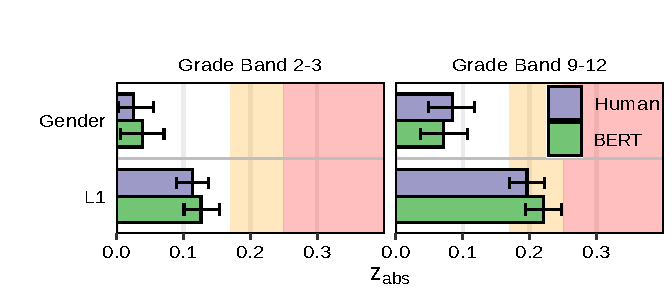
\includegraphics[width=8.2cm]{figures/20230422_ETS-DIF_zabs_ovr_edit.pdf}
    \caption{Estimates of overall DIF. Error bars indicate 95\% confidence intervals. Yellow shaded regions correspond to moderate DIF, and red shaded regions correspond to strong DIF.}
    \label{fig:zabs_ovr}
\end{figure}

\noindent \textbf{Human vs. BERT overall DIF} \;
Overall DIF of automated scores was highly similar to human scores. As seen in Figure \ref{fig:zabs_ovr}, green bars (representing BERT scores) are nearly commensurate with gray bars (representing human scores), with mostly overlapping 95\% confidence intervals. Yet, there was significantly more DIF in BERT scores compared to human scores with respect to L1 in Grade Band 9–12 ($\Delta z_{abs} = .025, CI_{95\%} = [.011, .039], p = 3.3 \cdot 10^{-4}$). In practical terms, however, an effect size of 0.025 standard deviations is very small. 

\noindent \textbf{Human vs. BERT individual item DIF} \;
In addition to overall DIF, we examined DIF of each individual item. Figure \ref{fig:zabs_itm} presents DIF of human and automated scores, for gender and L1, across Items 1–3, for each grade band. Human and automated scores are again quite consistent. For Grade Band 9–12, L1 DIF tends to be higher across all items; however, only Item 3 reaches statistical significance ($\Delta z_{abs} = .032, CI_{95\%} = [.010, .055], p = 3.3 \cdot 10^{-3}$). An effect size of 0.032 is very small.

\begin{figure}[h]
    \centering
    \hspace{-.6cm}
    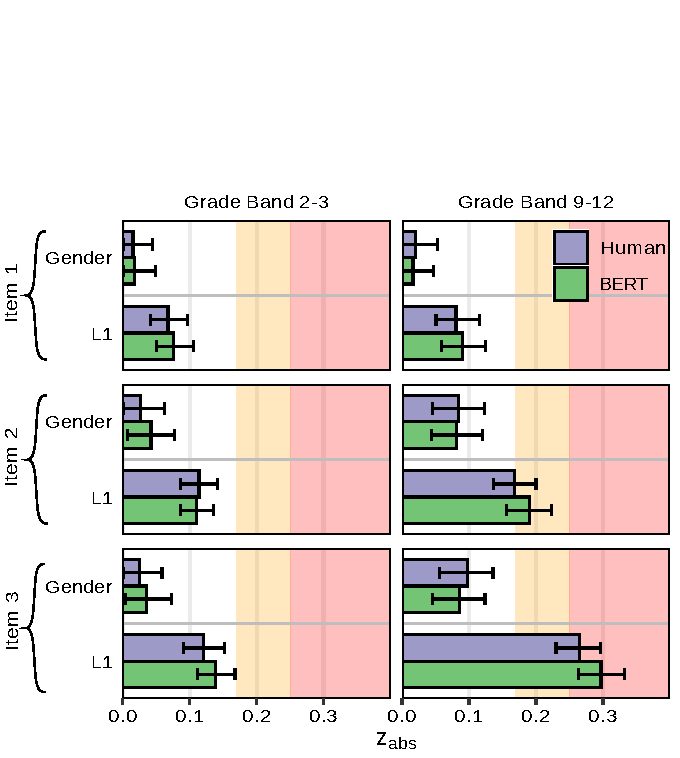
\includegraphics[width=8.2cm]{figures/20230422_ETS-DIF_zabs_itm_edit.pdf}
    \caption{Estimates of DIF for each of the 3 speaking items. Error bars indicate 95\% confidence intervals. Yellow shaded regions correspond to moderate DIF, and red shaded regions correspond to strong DIF.}
    \label{fig:zabs_itm}
\end{figure}

% % For adding bigger figures (across both columns)
% \begin{figure*}[htbp]
%     \centering
%     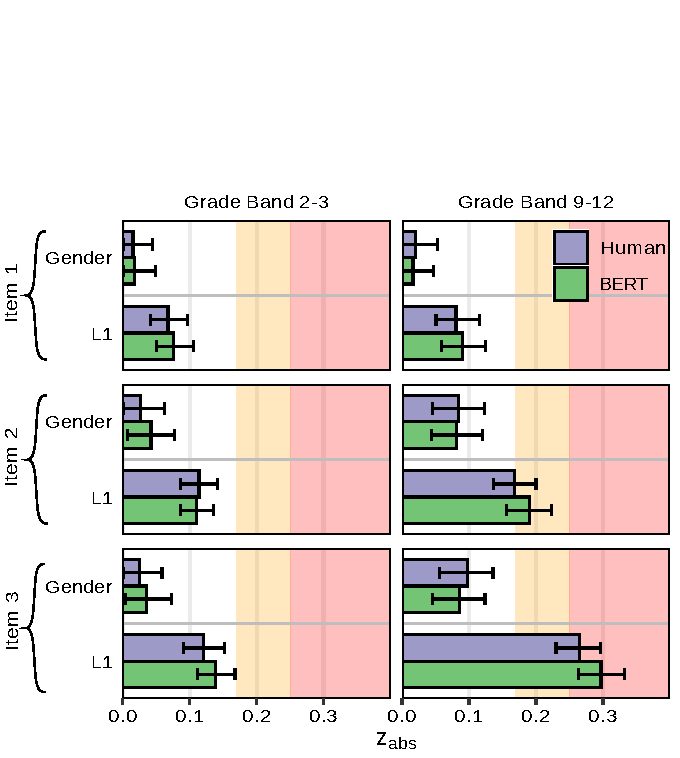
\includegraphics[width=16cm]{figures/20230422_ETS-DIF_zabs_itm_edit.pdf}
%     \caption{Estimates of DIF by gender and L1 for each of the 3 speaking items in grade-bands 2–3 and 9–12. Error bars indicate 95\% confidence intervals. Yellow shaded regions correspond to moderate DIF ($.17 < z_{abs} < .25$), and red shaded regions correspond to strong DIF ($z_{abs} > .25$).}
%     \label{fig:test}
% \end{figure*}

\subsection{DIF increases with item length}

Longer speaking items tended to exhibit more DIF than shorter speaking items. Automated scores, however, do not exacerbate this trend. 

In terms of item length, Item 3 was longer than Item 2, which was in turn longer than Item 1. Figure \ref{fig:zabs_itm} shows that DIF, too, generally increased in magnitude across items 1–3. Table \ref{itm_diff} presents the specific values of $\Delta z_{abs,ij}$ for all three item comparisons (corresponding to combinations of Item $i \neq j$) for each grade-band. 

\begin{table*}[ht]
\centering
\small  % comment out this line if wanted bigger font size
\begin{tabular}{lccccccc}
\toprule
    & \multicolumn{3}{c}{\textbf{Grade Band 2-3}} & \multicolumn{1}{c}{ } & \multicolumn{3}{c}{\textbf{Grade Band 9-12}} \\
    \cline{2-4}
    \cline{6-8}
    \textbf{Factor} & \textbf{2 - 1} & \textbf{3 - 1} & \textbf{3 - 2} & & \textbf{2 - 1} & \textbf{3 - 1} & \textbf{3 - 2} \\
    \midrule
    \multirow{2}*{Gender} & .012 & .010 & -.002 & & .065 * & .078 * & .013 \\
    & [-.030, .051] & [-.029, .049] & [-.042, .039] & & [.021, .110] & [.031, .116] & [-.032, .055] \\
    \multirow{2}*{L1} & .046 * & .053 * & .006 & & .087 * & .184 * & .097 * \\
    & [.009, .085] & [.010, .093] & [-.035, .046] & & [.043, .130] & [.139, .226] & [.056, .138] \\
    \bottomrule
    \end{tabular}
\caption{\label{itm_diff}
Differences in DIF between longer and shorter items, within each grade band, based on human ratings. "*" indicates that an estimate is statistically significant using B-H adjusted p-values. 95\% confidence intervals are presented in square brackets.}
\end{table*}

Although longer items tend to have more DIF, this general trend was not uniformly consistent across factors and grade-bands. Specifically, the trend was less consistent for gender: There were no statistically significant differences in Grade Band 2–3; and in Grade Band 9–12, Item 3 did not have more DIF than Item 2 at a statistically significant level. Additionally, for Grade Band 2–3, Item 3 did not have significantly more DIF than Item 2.

In order to determine if item-item differences were exacerbated by automated scoring, we computed second-order differences, $\Delta \Delta z_{abs}$. None of these values, however, were statistically significant. We conclude that the pattern of longer-items producing more DIF is consistent for both human and automated raters. 

\subsection{DIF is higher for older examinees}

In general, there is more DIF for older examinees (in Grade Band 9–12) compared to younger examinees (in Grade Band 2–3). Automated scores, however, do not exacerbate this trend.

There is significantly more DIF for Grade Band 9–12 compared to 2–3, in terms of both gender and L1. This trend can be seen clearly in Figure \ref{fig:zabs_itm}. Based on bootstrapped estimates for gender, $\Delta z_{abs} = .059$ ($CI_{95\%} = [.011, .100], p = 4.9 \cdot 10^{-3}$); and for L1, $\Delta z_{abs} = 0.082$ ($CI_{95\%} = [0.047, 0.120], p = 3.8 \cdot 10^{-6}$). 

When we examine individual items, this trend is present for items that are medium–long (Items 2 and 3) but not for short items (Item 1). Visually, this can be seen in Figure \ref{fig:zabs_itm}. Numerically, this is presented for human ratings in Table \ref{gr_diff}. 


\begin{table}[htbp]
\centering
\small  % comment out this line if wanted bigger font size
\begin{tabular}{p{0.8cm}ccc}
\toprule
\textbf{Factor} & \textbf{Item 1} & \textbf{Item 2} & \textbf{Item 3} \\
\midrule
\multirow{2}*{Gender} & .005 & .058 * & .072 * \\
            & [-.033, .042] & [.011, .105] & [.019, .118]\\
\multirow{2}*{L1} & .013   & .054 *  & .145 *  \\
 & [-.029, .057] & [.012, .098] & [.098, .193] \\
\bottomrule
\end{tabular}
\caption{\label{gr_diff}
Differences in DIF between grade-bands, based on human ratings, for each of the three speaking items. "*" indicates that an estimate is statistically significant using B-H adjusted p-values. 95\% confidence intervals are provided in square brackets.}
\end{table}

In order to determine if differences between grade-bands were exacerbated by automated scoring, we computed second-order differences, $\Delta \Delta z_{abs}$. None of these values, however, were statistically significant. We conclude that the trend of greater DIF in older examinees is consistent for both human and automated raters. 

\subsection{Severity of DIF depends on L1 and grade-band}

The magnitude and quantity of DIF varied by L1 background, and patterns were generally not consistent across grade-bands. Figure \ref{fig:z_ovr} depicts the magnitude and direction of DIF for gender and all L1 groups. For Grade Band 2–3, native speakers of Marshallese and Mayan languages showed evidence of moderate–strong DIF for human and BERT scores. DIF was negative for both L1 groups, indicating that these examinees fared worse on speaking items than their (equally-proficient) Spanish-speaking counterparts. 

\begin{figure*}[t]
    \centering
    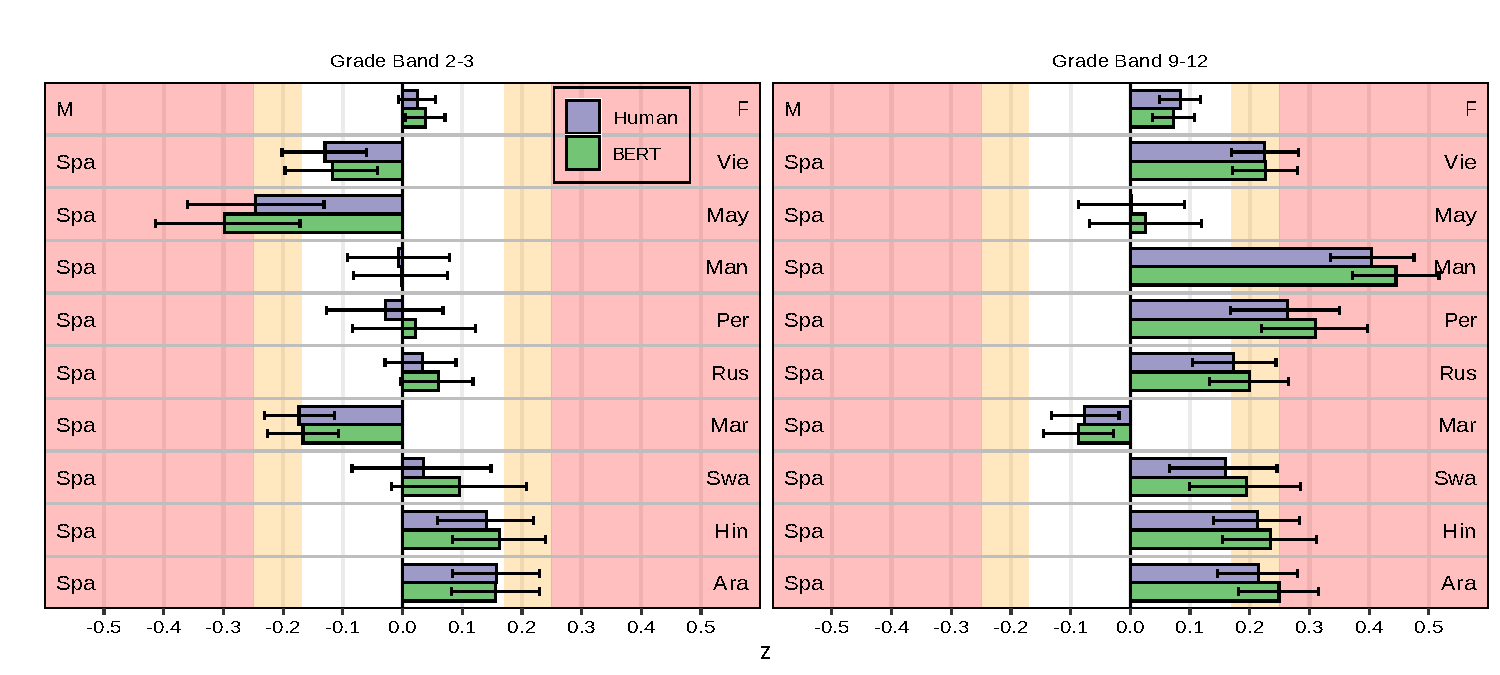
\includegraphics[width=16cm]{figures/20230422_ETS-DIF_z_ovr_edit.pdf}
    \caption{Estimates of direction and magnitude of overall DIF. Error bars indicate 95\% confidence intervals. Yellow shaded regions correspond to moderate DIF, and red shaded regions correspond to strong DIF. Reference groups are listed on the left of each chart (M = Male, Spa = Spanish); focal groups are listed on the right (L1 groups are abbreviated by the first three letters). DIF in the positive direction indicates that the focal group is favored.}
    \label{fig:z_ovr}
\end{figure*}

In Grade Band 9–12, examinees of nearly all L1 backgrounds fared better than native Spanish speakers. In this case, speaking items tended to disadvantage members of the reference group (i.e. examinees with Spanish L1 backgrounds). 

As with preceding analyses, DIF based on BERT scores aligned closely with DIF based on human scores. Although results showed that BERT exacerbated DIF in L1 as a whole (Section \ref{res_rq1}), analyses of individual L1 groups did not reveal any statistically significant differences between human and BERT scores. We also did not find any statistically significant differences between human and BERT scores when examining DIF at the individual item level (Appendix \ref{sec:appendix_z_itm}). 

\chapter{Discussion}

\subsection{Main findings}

Analysis of differential item functioning (DIF) revealed specific patterns of biases in human and automated scores of English speaking assessment. With respect to human scores, we found that there was more DIF for older examinees and for longer items. Based on commonly accepted standards regarding effect size, there was a moderate amount of overall DIF in Grade Band 9–12 based on examinees’ native language (L1) backgrounds. Automated scores generated by off-the-shelf BERT models closely matched human scores, yet BERT was found to exacerbate overall DIF for Grade Band 9–12 based on examinees’ native language (L1). The degree to which BERT exacerbated this bias, however, was very small.

\subsection{Causes of DIF}

Although our findings do not confirm any causes of DIF, they do allow us to rule out several possibilities. 

\noindent \textbf{Implicit bias} \;
Our automated scoring system was based exclusively on transcripts of examinees’ speech. No phonic information was used in the automated scoring process. It is notable, then, that there was no mitigation of DIF in automated scores using a text-based BERT model. In other words, removal of acoustic input did not reduce bias. From this, we conclude that examinees with \emph{identical} (transcribed) responses could not have received higher or lower scores, on average, based on gender or L1. 

Although text-based automated scores did not mitigate bias, this does not necessarily imply that human raters were unaffected by implicit bias. It is possible, for instance, that examinees with different accents also had different (transcribed) responses, which still affected human raters' judgment. 

\noindent \textbf{Transcription (in)accuracy} \;
Prior research shows that there are discrepancies in word error rate (WER) of automated transcription based on L1 (Anonymous). Specifically, automated transcription struggles with speakers of Vietnamese L1 backgrounds. Yet given the close correspondence between human and automated scores—for all examinees, not just Vietnamese examinees—it appears unlikely that transcription inaccuracies engender lower or higher scores. 

\subsection{Accuracy and DIF}

As the performance of automated scoring improves to match (or exceed) that of human raters, one might expect the magnitude of DIF to also match (or potentially reduce) that of human raters. For longer speaking items, however, we found that automated scores exceeded the performance of human raters, yet increased DIF. More research is needed to determine the relationship between performance of automated scoring systems and DIF.

\subsection{Limitations}

Our analyses are based around one metric of uniform DIF, $z$. The benefits of $z$ are that it is commonly used in practice, it is highly interpretable with well-established effect sizes, and it is easy to aggregate across items and focal groups. One of the drawbacks, however, is that it does not capture non-uniform DIF, and it is not ideal in terms of statistical power \citep{woods2013}. 

Consistent with other analyses of DIF, our study struggles to identify sources of DIF \citep{zumbo2007}. Although it is outside the scope of this study, a fine-grained analysis of examinees’ language, especially based on L1, could provide insight. Additionally, it could be beneficial to explore the possibility of modifying BERT using debiasing techniques \citep{sun2019mitigating}. Not only could these techniques potentially reveal sources of DIF, but they may be able to reduce DIF of human raters.

\chapter{Appendices}

\section{L1 Groups}
\label{sec:appendix_lang}

In selecting L1 groups, one of our aims was to represent languages from around the globe. In some cases, this required grouping languages to reach an adequate sample size for statistical analyses. Given the constraints of sample size, we tried to ensure that L1 groups were as geo-historically related to each other as possible \citep{brown2005encyclopedia}. The four composite L1 groups in our study were (1) Hindi, (2) Mayan languages, (3) Persian, and (4) Swahili. For simplicity, we refer to composite L1 groups by the predominate language within each group, with the exception of Hindi (in order to remain consistent with a prior study). It would be more accurate, however, to refer to the L1 groups as (1) Indo-Aryan, (2) Indigenous languages of Central and South America, (3) Indo-European languages of the Middle East, and (4) Niger-Congo languages. 

The languages within each of the composite L1 groups are presented in Table \ref{lang_grp}. Note that the names of languages are derived from states’ departments of education, which do not follow the same naming conventions. We made minor changes in compiling the list of languages (e.g. changing “Panjabi” to “Punjabi”). 

\begin{table*}[htbp]
\centering
% \small  % comment out this line if wanted bigger font size
\begin{tabular}{lccccccc}
\toprule
    & \multicolumn{2}{c}{\textbf{Grade Band 2-3}} & \multicolumn{1}{c}{ } & \multicolumn{2}{c}{\textbf{Grade Band 9-12}} \\
    \cline{2-3}
    \cline{5-6}
     \textbf{Language} & \textbf{n} & \textbf{\%} & & \textbf{n} & \textbf{\%} \\
    \midrule
\textbf{Hindi} & & & & & \\
\hspace{3mm} Punjabi & 157 & 37.7 & & 75 & 40.5 \\
\hspace{3mm} Hindi & 124 & 29.8 & & 39 & 21.1 \\
\hspace{3mm} Urdu & 65 & 15.6 & & 35 & 18.9 \\
\hspace{3mm} Gujarati & 46 & 11.1 & & 30 & 16.2 \\
\hspace{3mm} Marathi & 24 & 5.8 & & 6 & 3.2 \\
\textbf{Mayan languages} & & & & & \\
\hspace{3mm} Mayan languages & 212 & 89.1 & & 214 & 82.9 \\
\hspace{3mm} Q'anjob'al & 24 & 10.1 & & 40 & 15.5 \\
\hspace{3mm} Quechua & 1 & 0.4 & & 3 & 1.2 \\
\hspace{3mm} Q'eqchi & 1 & 0.4 & & 1 & 0.4 \\
\textbf{Persian} & & & & & \\
\hspace{3mm} Persian & 209 & 70.8 & & 97 & 49.2 \\
\hspace{3mm} Kurdish & 76 & 25.8 & & 87 & 44.2 \\
\hspace{3mm} Farsi & 10 & 3.4 & & 13 & 6.6 \\
\textbf{Swahili} & & & & & \\
\hspace{3mm} Swahili & 89 & 42.6 & & 120 & 55.3 \\
\hspace{3mm} Nuer & 37 & 17.7 & & 28 & 12.9 \\
\hspace{3mm} Niger-Kordofanian languages & 16 & 7.7 & & 16 & 7.4 \\
\hspace{3mm} Dinka & 19 & 9.1 & & 11 & 5.1 \\
\hspace{3mm} Kinyarwanda & 7 & 3.3 & & 19 & 8.8 \\
\hspace{3mm} Wolof & 15 & 7.2 & & 10 & 4.6 \\
\hspace{3mm} Fulah & 10 & 4.8 & & 5 & 2.3 \\
\hspace{3mm} Igbo & 7 & 3.3 & & 5 & 2.3 \\
\hspace{3mm} Yoruba & 3 & 1.4 & & 1 & 0.5 \\
\hspace{3mm} Hausa & 1 & 0.5 & & 1 & 0.5 \\
\hspace{3mm} Akan & 2 & 1 & & 0 & 0 \\
\hspace{3mm} Shona & 2 & 1 & & 0 & 0 \\
\hspace{3mm} Chichewa; Chewa; Nyanja & 0 & 0 & & 1 & 0.5 \\
\hspace{3mm} Kirundi & 1 & 0.5 & & 0 & 0 \\
    \bottomrule
    \end{tabular}
\caption{\label{lang_grp}
Languages of composite L1 groups by grade-band.}
\end{table*}

There is a great deal of heterogeneity within L1 groups, as with gender, and as with all other demographic characteristics. We note that L1 is not synonymous with cultural identity, racial identity, geographic identity, or preferred language. Despite these limitation, in the context of English speech assessment, we believe L1 is a more relevant construct than, say, conventional racial categories (e.g. White, Asian, Black). 

\section{BERT Performance Metrics}
\label{sec:appendix_perf}

Performance metrics of all six BERT models are presented in Table \ref{bert_perf}. Approximately 10\% of all responses were scored by two human raters, independently, which provides the basis for comparisons between human and BERT performance. 

\begin{table*}[ht]
\centering
\small  % comment out this line if wanted bigger font size
\begin{tabular}{lccccccccccccc}
\toprule
    & \multicolumn{6}{c}{\textbf{Grade Band 2-3}} & \multicolumn{1}{c}{ } & \multicolumn{6}{c}{\textbf{Grade Band 9-12}} \\
    \cline{2-7}
    \cline{9-14}
    & \multicolumn{2}{c}{\textbf{Acc.}} & \multicolumn{2}{c}{\textbf{r}} & \multicolumn{2}{c}{\textbf{QWK}} & \multicolumn{1}{c}{ } & \multicolumn{2}{c}{\textbf{Acc.}} & \multicolumn{2}{c}{\textbf{r}} & \multicolumn{2}{c}{\textbf{QWK}} \\
    \textbf{Item} & \textbf{Human} & \textbf{BERT} & \textbf{Human} & \textbf{BERT} & \textbf{Human} & \textbf{BERT} & & \textbf{Human} & \textbf{BERT} & \textbf{Human} & \textbf{BERT} & \textbf{Human} & \textbf{BERT} \\
    \midrule
    1 & .911 & .896 & .793 & .713 & .792 & .713 & & .929 & .904 & .920 & .895 & .920 & .895 \\
    2 & .756 & .685 & .898 & .861 & .898 & .859 & & .728 & .700 & .911 & .910 & .911 & .909 \\
    3 & .614 & .618 & .834 & .834 & .834 & .829 & & .694 & .707 & .841 & .885 & .609 & .884 \\
    \bottomrule
    \end{tabular}
\caption{\label{bert_perf}
 “human” refers to human-human comparisons. The number of observations that were scored by two human raters ranges from 1,567–1641 for Grade Band 2–3, and from 1,254–1,293 for Grade Band 9–12. “BERT” refers to human-BERT comparisons. The number of observations in the testing sets were 4,185 for Grade Band 2–3, and 3,306 for Grade Band 9–12.}
\end{table*}

\section{Human vs. BERT DIF for each item}
\label{sec:appendix_z_itm}

Figure \ref{fig:z_itm} presents the magnitude and direction of DIF of Items 1-3 for grade-bands 2-3 and 9-12, based on gender and all nine L1 focal groups separately.

\begin{figure*}[t]
    \centering
    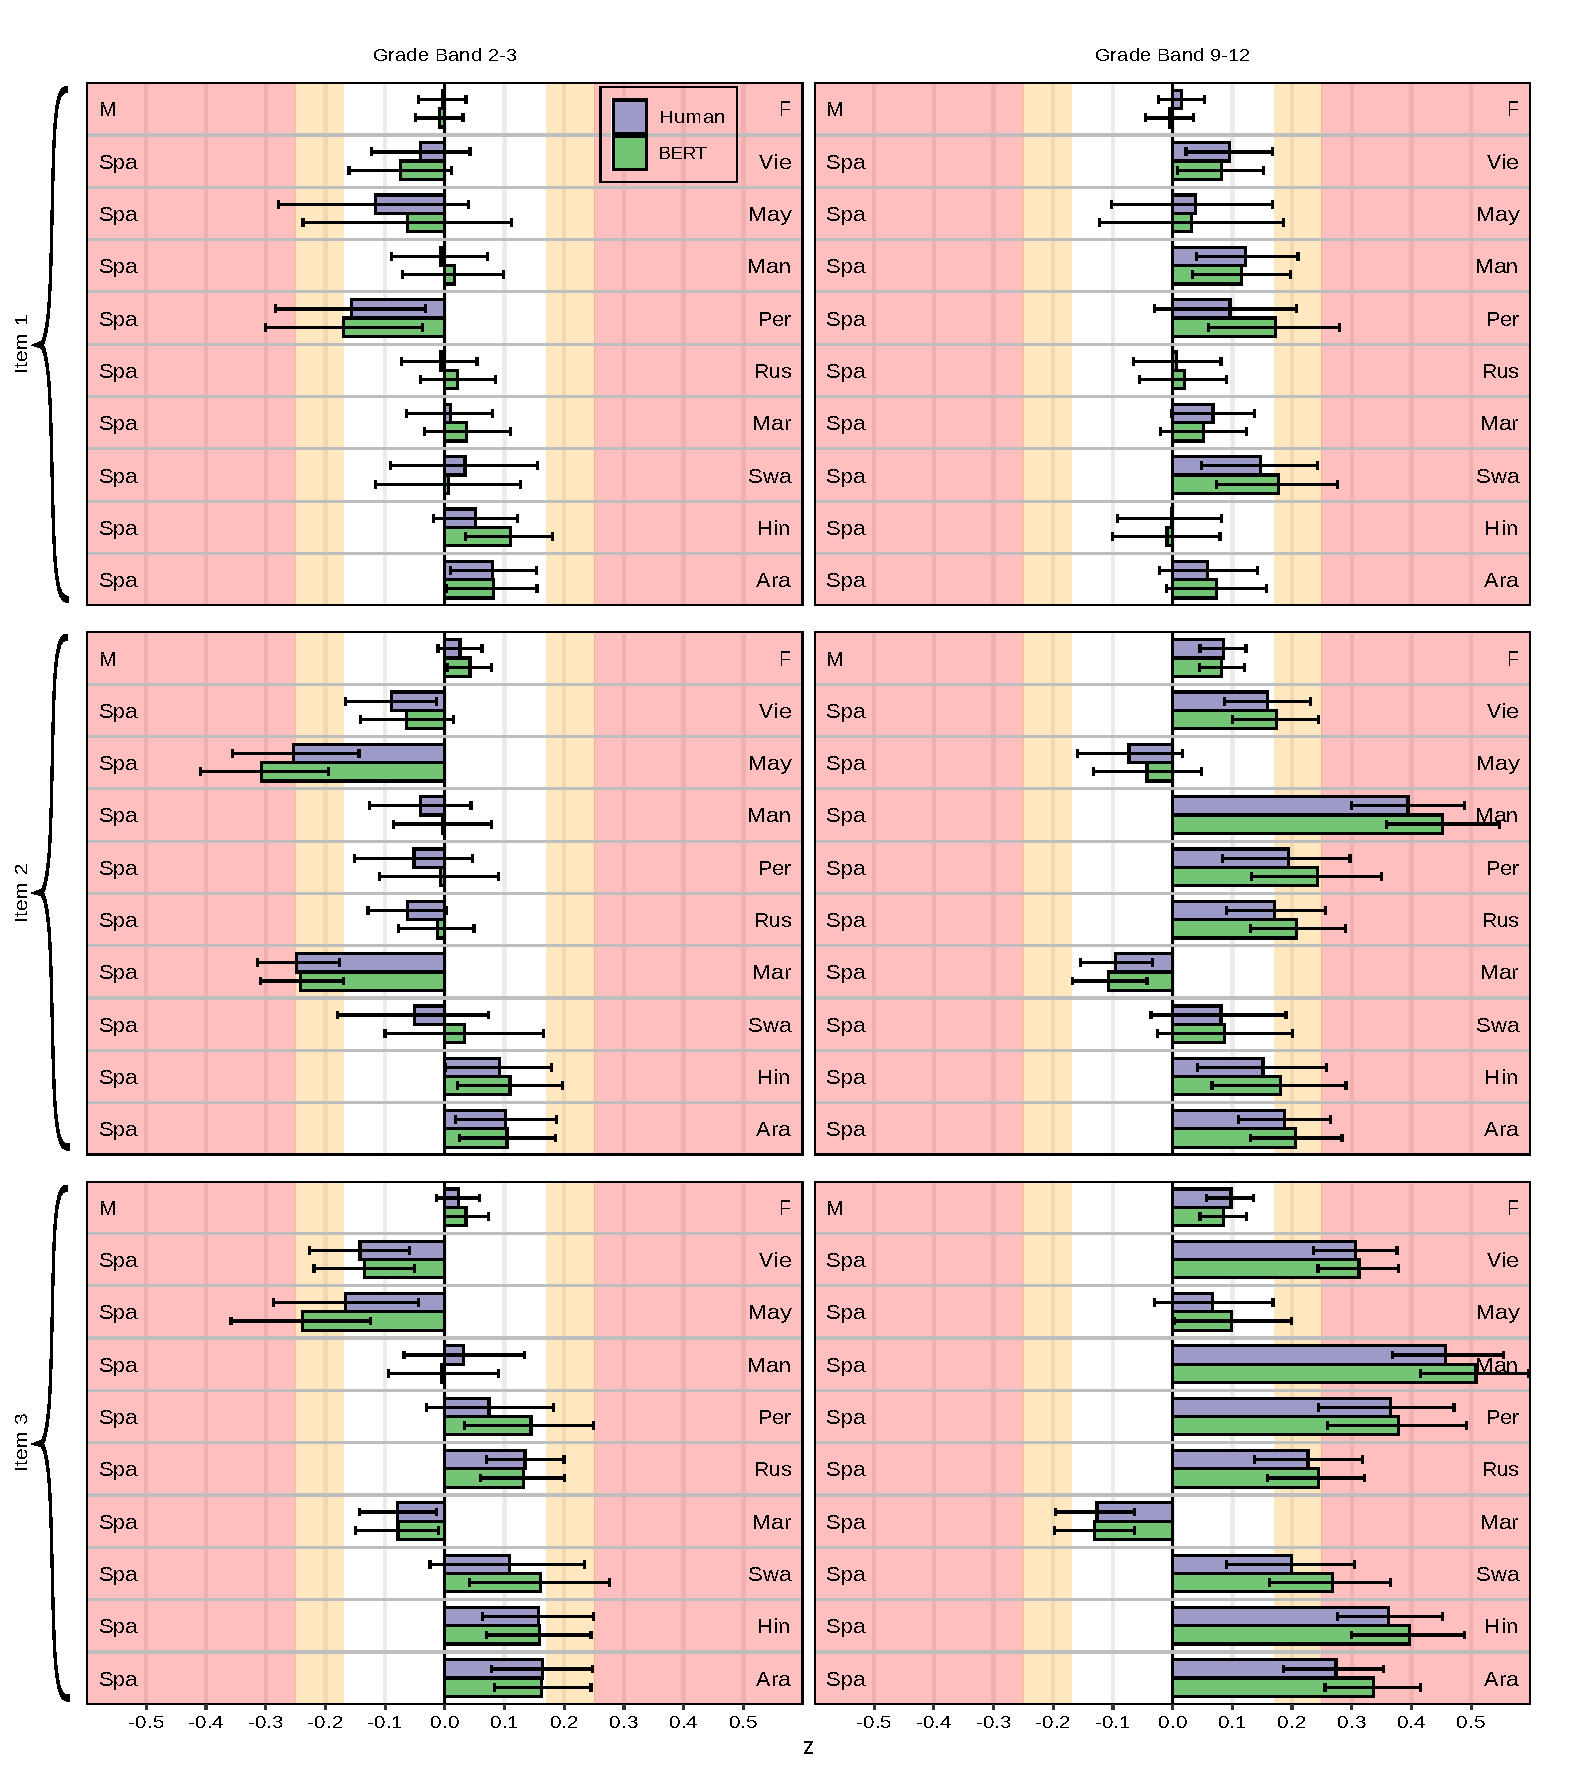
\includegraphics[width=16cm]{figures/20230422_ETS-DIF_z_itm_edit.pdf}
    \caption{Estimates of direction and magnitude of DIF for each of the three speaking items. Error bars indicate 95\% confidence intervals. Yellow shaded regions correspond to moderate DIF, and red shaded regions correspond to strong DIF. Reference groups are listed on the left of each chart (M = Male, Spa = Spanish); focal groups are listed on the right (L1 groups are abbreviated by the first three letters). DIF in the positive direction indicates that the focal group is favored.}
    \label{fig:z_itm}
\end{figure*}

%\bibliography {bib/network,bib/naming}    % bibliography references
\bibliography{20230507_dissertation}
%\bibliographystyle {thesis}
%\bibliographystyle{apa-like}
%\bibliographystyle {uclathes}
%\bibliographystyle{apalike}
%\bibliographystyle{acl_natbib}
\bibliographystyle{plainnat}

\end {document}

